
\chapter{Results}
\label{chapt:results}

We will evaluate three algorithms in this section:
the algorithm that was used when I arrived in the Megason Lab (see subsection~\ref{sect:megasonExisting}),
the variant of the Laplacian of Gaussian presented in \cite{al2009improved} : scale constrained Laplacian of Gaussian (see subsection~\ref{sect:farsight}),
and our proposed algorithm (see chapter~\ref{chapt:proposal}).



%%%%%%%%%%%%%%%%%%%%%%%%%%%%%%%%%%%%%%%%%%%%%%%%%%%%%%%%%%%%%%%%%%%%%%%%%%%%%%%
%%%%%%%%%%%%%%%%%%%%%%%%%%%%%%%%%%%%%%%%%%%%%%%%%%%%%%%%%%%%%%%%%%%%%%%%%%%%%%%
%%%%%%%%%%%%%%%%%%%%%%%%%%%%%%%%%%%%%%%%%%%%%%%%%%%%%%%%%%%%%%%%%%%%%%%%%%%%%%%



\section{Evaluation framework}

The evaluation is performed both on synthetic and real data. We provide information about the detection quality, the robustness, and the processing time of each algorithm.

\subsection{Evaluation data}

The data presented in this section is illustrated in the annex~\ref{annex:EvalData}.

\subsubsection{Synthetic data}

Synthetic data was provided for evaluating the robustness of algorithms.
The data set consists into 10 3D images containing noisy nuclei and membrane channels.
The datasets are non isotropic, and the resolution along z is 5 times the resolution along x and y.
The amount of nuclei goes from 100 to 1000, with increasing level of noise.

This dataset is very useful for testing robustness to noise and anisotropy, but it does not include stacked nuclei.


\subsubsection{Real data}

\begin{figure}[htb]
\begin{center}
\leavevmode
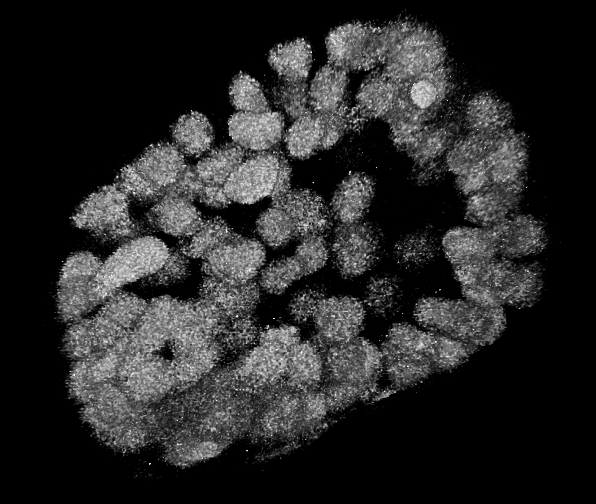
\includegraphics[width=0.6\textwidth]{pictures/rawRaycast}
\end{center}
\caption{3D rendering by ray tracing of the nuclei channel of the real dataset used for evaluation.}
\label{fig:rawRaycast}
\end{figure}

The real data corresponds to 3D dataset of the ear of a zebrafish embryo (see figure~\ref{fig:rawRaycast}).
It consists in a membrane and nuclei channel, and a manual segmentation of nuclei in a region of the image.
There are 141 nuclei in the manually segmented region of the dataset. 

\subsection{Evaluation criterion}

We evaluate:
\begin{itemize}
\item the number of correctly detected nuclei, which correspond to one detection in a manually segmented nuclei,
\item the number of outside detections corresponding to detections of nuclei outside of manually segmented nuclei.
\item the number of over-detection corresponding to re-detection of an already detected nuclei (two or more detections inside a cell nuclei).
\item "success" which corresponds to:\\
 \[
 \frac{correctly detected}{undetected + over detected + outside detections + correctly detected} 
 \]
\end{itemize} 

We also evaluate the processing time of the algorithms using information provided by the unix 'time' command, as it is able to give the time spent by each cpu on the processing task, making the implementation less determinant for the evaluation.


%%%%%%%%%%%%%%%%%%%%%%%%%%%%%%%%%%%%%%%%%%%%%%%%%%%%%%%%%%%%%%%%%%%%%%%%%%%%%%%
%%%%%%%%%%%%%%%%%%%%%%%%%%%%%%%%%%%%%%%%%%%%%%%%%%%%%%%%%%%%%%%%%%%%%%%%%%%%%%%
%%%%%%%%%%%%%%%%%%%%%%%%%%%%%%%%%%%%%%%%%%%%%%%%%%%%%%%%%%%%%%%%%%%%%%%%%%%%%%%


\section{Evaluation results}


\subsection{Evaluation on synthetic data}

The evaluation results are detailed in annex~ref{annex:Eval}. We present here the "success" percentage of the algorithms (see tabular~\ref{tab:simuSuccess}).
\begin{figure}[htb]
\begin{center}
\subfloat[][]{
\begin{tabular}{|l|l|}
\hline Algorithm & Success (\%) \\ 
\hline Existing algorithm in Megason Lab & 40 \\ 
\hline Scale constrained Laplacian of Gaussian & 98 \\ 
\hline Proposal & 99 \\ 
\hline
\end{tabular}\label{tab:meanSuccess}}\\
%
\subfloat[][]{
\begin{tabular}{|l|l|}
\hline Algorithm & Success (\%) \\ 
\hline Existing algorithm in Megason Lab & 7 \\ 
\hline Scale constrained Laplacian of Gaussian &  93 \\ 
\hline Proposal & 95 \\ 
\hline
\end{tabular}\label{tab:hardSuccess}}
\end{center}
\caption{Evaluation of 3 algorithms on 10 synthetic datasets of increasing difficulty:\\
\subref{tab:meanSuccess} presents the mean value of "success" over the 10 synthetic datasets containing 100 to 1000 cells.
\subref{tab:hardSuccess} presents the "success" on the hardest dataset, very noisy and containing 1000 cells.
}
\label{tab:simuSuccess}
\end{figure}
The evaluation on synthetic data proved the proposed algorithm to have the highest "success" percentage,
meaning that it detects more nuclei without mistakes. Then comes the scale constrained Laplacian of Gaussian which is very robust
but has more detections outside of nuclei than the proposed algorithm. Finally the existing algorithm performs worse than the two others,
after a certain amount of noise in the images.


\subsubsection{Evaluation a segmented dataset}

We present here the results of the evaluation on a real 2-photon/confocal dataset (see tabular~\ref{tab:realEval}). We can see that all algorithm preforms poorly on this dataset.
The difficulties mentioned in section~\ref{setc:ChallengesData}, makes this dataset very hard to process. Another difficulty is the particular shape of the cells in this region: they are elongated, and nuclei are most of times located next to the border of the cells.
This evaluation let us compare the three algorithms on a very hard dataset.
\begin{figure}[htb]
\begin{center}
\begin{tabular}{|p{2.5cm}|l|l|p{1.3cm}|l|}
\hline Algorithm & Correct (\%) & Outside (\%) & Over-detected (\%) & Success (\%) \\ 
\hline Existing algorithm in Megason Lab & 50 & 40 & 26 & 30 \\ 
\hline Scale constrained Laplacian of Gaussian &  74 & 36 & 6 & 51 \\ 
\hline Proposal & 60 & 30 & 2 & 48 \\
\hline
\end{tabular}
\end{center}
\caption{Evaluation of 3 algorithms on a real dataset of the ear of a zebrafish embryo. the results are normalized by the number of cells in the image.}
\label{tab:realEval}
\end{figure}

We can see that the Scale constrained Laplacian of Gaussian outperforms both existing and presented algorithms in terms of detected cells.
It is also important to notice that it make more outside of nuclei and over-detections than the proposed algorithm.
The existing algorithm performs worse than the two others.


\subsection{Time evaluation}

We computed the execution time of the three algorithms, on the real dataset (see tabular~\ref{tab:timeEval}
\begin{figure}[htb]
\begin{center}
\begin{tabular}{|l|l|}
\hline Algorithm & Processing time (min) \\ 
\hline Existing algorithm in Megason Lab & 16 \\ 
\hline Scale constrained Laplacian of Gaussian &  22 \\ 
\hline Proposal & 21 \\
\hline
\end{tabular}
\end{center}
\caption{Processing time of 3 algorithms on a real dataset of 1024x1024x57 voxels. Inputs are raw nuclei and membrane channels.}
\label{tab:timeEval}
\end{figure}
The fastest algorithm is the one currently used in the Megason lab, with an execution time of 16 minutes.
Then the Laplacian of Gaussian and the Proposal have approximatively the same processing time.
We decided to focus on algorithms rather than implementation, so the given times is the sum of the time spent by each computer,
thus, we don't advantage too much the multi-threaded implementations.



%%%%%%%%%%%%%%%%%%%%%%%%%%%%%%%%%%%%%%%%%%%%%%%%%%%%%%%%%%%%%%%%%%%%%%%%%%%%%%%
%%%%%%%%%%%%%%%%%%%%%%%%%%%%%%%%%%%%%%%%%%%%%%%%%%%%%%%%%%%%%%%%%%%%%%%%%%%%%%%
%%%%%%%%%%%%%%%%%%%%%%%%%%%%%%%%%%%%%%%%%%%%%%%%%%%%%%%%%%%%%%%%%%%%%%%%%%%%%%%


\section{Implementation details}

The data we are processing are 3D plus time, this represents huge datasets, that are hardly processed by Matlab.
Thus, prototyping was done in {\C++}, using medical image processing libraries such as the Insight ToolKit (ITK)
or the Visualization ToolKit (VTK).

\subsection{Programmation language and libraries}

The algorithms developed in the Megason lab are directly used by Biologists on a day to day basis.
They are integrated to the program developed by a group of computer scientists (Arnaud Gelas, Lydie Souhait and Nicolas Rannou): {\gofigure}.
This program is exclusively coded in \C++ and integrates ITK and VTK.
Our algorithm must be coded in such way that this group can reuse them and integrate them (abundant documentation and accessibility to source code).

The use of ITK give us the opportunity to develop fast algorithms, able to process huge datasets, but it also adds a lot of complexity to the prototyping process.


\subsection{Reproducibility}

All developed algorithms but Kishore's are open source and distributed on the internet, on \href{http://github.com/antonin07130}{Github}.
This provides other computer scientists with the opportunity to download and compile the programs I created.
Those are open source and cross platform. The proposed algorithm consists in a series of small programs linked by a bash script.


%%%%%%%%%%%%%%%%%%%%%%%%%%%%%%%%%%%%%%%%%%%%%%%%%%%%%%%%%%%%%%%%%%%%%%%%%%%%%%%
%%%%%%%%%%%%%%%%%%%%%%%%%%%%%%%%%%%%%%%%%%%%%%%%%%%%%%%%%%%%%%%%%%%%%%%%%%%%%%%
%%%%%%%%%%%%%%%%%%%%%%%%%%%%%%%%%%%%%%%%%%%%%%%%%%%%%%%%%%%%%%%%%%%%%%%%%%%%%%%

\section{Conclusion}

We can see that the proposed algorithm, processing mainly the membrane information, outperforms the existing algorithm in the Megason Lab.
The scale constrained Laplacian of Gaussian performs better than those two algorithms for detecting seeds, but also produces more false detections
(over detections and out of nuclei detections).
It is important to notice that the real dataset is a special arrangement of cells, and it would be important to test the algorithms on a different dataset. Also, this dataset has been masked by a "region of interest", in such way that all membranes facing outer parts of the region were left open leading to detection of nuclei out of the region of interest.
It is also hard to compare those results directly with those of articles which evaluate their algorithms after the segmentation, as most of them use a segmentation refinement step,
for eliminating objects that are segmented but do not correspond to nuclei in terms of shape characteristics.
A visual comparison showed us that in case of stacked nuclei, our proposal was able to correctly separate nuclei when the two other algorithm would fail. It is unfortunately hard to display such results\footnote{
I created two applications for this purpose that can be found on Github:
\begin{description}
\item[\href{http://github.com/antonin07130/itkCompareProject}{Compare Project}]: which is useful for comparing two itk images slice by slice, especially "compareguiexample" which provides a GUI for visualizing and comparing such datasets.
\item[\href{http://github.com/antonin07130/SeedVisu}{SeedsVisualization}]: which takes a list of point and an itk 3D dataset as inputs. This programs renders the volume with a ray tracing algorithm, and superpose the points listed in the text file.
\end{description}
} in a paper format, as data are three dimensional and results are points within these datasets.

